\documentclass[10.5pt,a4paper]{article}
\usepackage[utf8]{vietnam}
\usepackage{amsmath,amssymb}
\usepackage{tabularx}
\usepackage{tikz}
\usetikzlibrary{calc}
\usepackage[top=0.9cm, bottom=0.9cm, left=1.1cm, right=1.1cm]{geometry}
\usepackage{fancyhdr}
\usepackage{enumitem}

\pagestyle{fancy}
\fancyhf{}
\rfoot{\small\textit{Trang \thepage/2}}
\lfoot{\small\textit{Đề kiểm tra Giữa học kì I -- Môn Toán 7 -- Đề 2}}
\renewcommand{\headrulewidth}{0pt}

\setlength{\parskip}{0.5pt}

\begin{document}

\noindent
\begin{tabularx}{\linewidth}{X r}
\textbf{TRƯỜNG THCS \dots\dots\dots\dots\dots\dots} & \textbf{ĐỀ KIỂM TRA GIỮA HỌC KÌ I -- NĂM HỌC 2026 -- 2027} \\
\textbf{TỔ: \dots\dots\dots\dots\dots\dots} & \textbf{Môn: TOÁN -- Lớp 7} \\
\textit{(Đề 2 -- gồm 02 trang)} & \textit{Thời gian làm bài: 90 phút (không kể thời gian giao đề)} \\
\end{tabularx}

\vspace{1mm}
\noindent
\fbox{\parbox{\dimexpr\linewidth-2\fboxsep-2\fboxrule\relax}{
\textbf{Họ và tên học sinh:} \dots\dots\dots\dots\dots\dots\dots\dots\dots\dots\dots\dots\dots\dots\dots \textbf{Lớp:} \dots\dots\dots \textbf{Số báo danh:} \dots\dots\dots
}}

\vspace{1.5mm}
\noindent\textbf{\large PHẦN I. Câu trắc nghiệm nhiều phương án lựa chọn (3,0 điểm).}
\vspace{0.5mm}

\noindent\textit{Thí sinh trả lời từ câu 1 đến câu 12. Mỗi câu hỏi thí sinh chỉ chọn một phương án.}

\vspace{1mm}
\noindent\textbf{Câu 1.} Tập hợp các số hữu tỉ được kí hiệu là\\
\begin{tabularx}{\linewidth}{X X X X}
A. $\mathbb{N}$ & B. $\mathbb{Z}$ & C. $\mathbb{Q}$ & D. $\mathbb{R}$
\end{tabularx}

\vspace{1mm}
\noindent\textbf{Câu 2.} Trong các số hữu tỉ $-\dfrac{2}{3}; \dfrac{1}{2}; -\dfrac{3}{4}; 0$, số nhỏ nhất là\\
\begin{tabularx}{\linewidth}{X X X X}
A. $-\dfrac{2}{3}$ & B. $-\dfrac{3}{4}$ & C. $0$ & D. $\dfrac{1}{2}$
\end{tabularx}

\vspace{1mm}
\noindent\textbf{Câu 3.} Với $x$ là số hữu tỉ, $(x^3)^4$ bằng\\
\begin{tabularx}{\linewidth}{X X X X}
A. $x^{12}$ & B. $x^7$ & C. $x^{81}$ & D. $x^{64}$
\end{tabularx}

\vspace{1mm}
\noindent\textbf{Câu 4.} Bỏ dấu ngoặc trong biểu thức $\dfrac{1}{3} - \left(\dfrac{1}{2} - \dfrac{1}{4}\right)$ ta được\\
\begin{tabularx}{\linewidth}{X X X X}
A. $\dfrac{1}{3} - \dfrac{1}{2} - \dfrac{1}{4}$ & B. $\dfrac{1}{3} + \dfrac{1}{2} - \dfrac{1}{4}$ & C. $\dfrac{1}{3} + \dfrac{1}{2} + \dfrac{1}{4}$ & D. $\dfrac{1}{3} - \dfrac{1}{2} + \dfrac{1}{4}$
\end{tabularx}

\vspace{1mm}
\noindent\textbf{Câu 5.} Số thập phân vô hạn tuần hoàn $2,1(6)$ có chu kì là\\
\begin{tabularx}{\linewidth}{X X X X}
A. $1$ & B. $16$ & C. $6$ & D. $21$
\end{tabularx}

\vspace{1mm}
\noindent\textbf{Câu 6.} Khẳng định nào sau đây đúng?\\
\begin{tabularx}{\linewidth}{X X X X}
A. $\sqrt{81} = -9$ & B. $\sqrt{81} = 9$ & C. $\sqrt{81} = \pm 9$ & D. $\sqrt{81} = 40,5$
\end{tabularx}

\vspace{1mm}
\noindent\textbf{Câu 7.} Giá trị tuyệt đối của số thực $-\sqrt{3}$ là\\
\begin{tabularx}{\linewidth}{X X X X}
A. $-\sqrt{3}$ & B. $3$ & C. $-3$ & D. $\sqrt{3}$
\end{tabularx}

\vspace{1mm}
\noindent\textbf{Câu 8.} Làm tròn số $-12,4578$ với độ chính xác $0,05$ ta được\\
\begin{tabularx}{\linewidth}{X X X X}
A. $-12,5$ & B. $-12,4$ & C. $-12,46$ & D. $-12,45$
\end{tabularx}

\vspace{1mm}
\noindent\textbf{Câu 9.} Tia $Oz$ là tia phân giác của góc $xOy$ khi\\
\begin{tabularx}{\linewidth}{X X}
A. $Oz \perp Ox$. & B. $Oz$ nằm giữa $Ox$ và $Oy$. \\
C. $Oz$ nằm giữa $Ox, Oy$ và $\widehat{xOz} = \widehat{zOy}$. & D. $\widehat{xOz} + \widehat{zOy} = \widehat{xOy}$.
\end{tabularx}

\vspace{1mm}
\noindent\textbf{Câu 10.} Đường thẳng $c$ cắt hai đường thẳng song song $a$ và $b$. Khẳng định nào sau đây đúng?\\
\begin{tabularx}{\linewidth}{X X}
A. Hai góc so le trong bù nhau. & B. Hai góc đồng vị bằng nhau. \\
C. Hai góc trong cùng phía bằng nhau. & D. Hai góc đồng vị bù nhau.
\end{tabularx}

\vspace{1mm}
\noindent
\begin{minipage}[m]{0.65\linewidth}
\textbf{Câu 11.} Cho hình bên, tia $Ot$ là tia phân giác của góc $xOy$ và $\widehat{xOy} = 130^\circ$. Số đo góc $xOt$ là\\
\begin{tabularx}{\linewidth}{X X}
A. $130^\circ$ & B. $50^\circ$ \\
C. $115^\circ$ & D. $65^\circ$
\end{tabularx}
\end{minipage}
\hfill
\begin{minipage}[m]{0.33\linewidth}
\centering
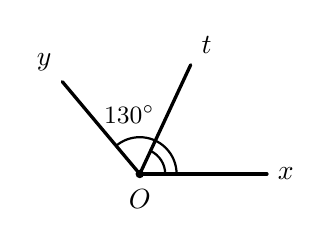
\begin{tikzpicture}[scale=0.85, line cap=round, line join=round]
  \coordinate (O) at (0,0);
  \coordinate (X) at (1.9,0);
  \coordinate (Y) at ({1.8*cos(130)}, {1.8*sin(130)});
  \coordinate (T) at ({1.8*cos(65)}, {1.8*sin(65)});
  \draw[very thick] (O) -- (X) node[right] {$x$};
  \draw[very thick] (O) -- (Y) node[above left] {$y$};
  \draw[very thick] (O) -- (T) node[above right] {$t$};
  \fill (O) circle (1.8pt) node[below=2pt] {$O$};
  \draw[thick] (0.55,0) arc (0:130:0.55);
  \draw[thick] (0.38,0) arc (0:65:0.38);
  \node at (100:0.9) {\small $130^\circ$};
\end{tikzpicture}
\end{minipage}

\vspace{1mm}
\noindent
\begin{minipage}[m]{0.65\linewidth}
\textbf{Câu 12.} Cho hình bên, đường thẳng $c$ cắt hai đường thẳng $a, b$ lần lượt tại $A, B$. Cặp góc nào sau đây là cặp góc đồng vị?\\
\begin{tabularx}{\linewidth}{X X}
A. $\widehat{A}_2$ và $\widehat{B}_2$ & B. $\widehat{A}_3$ và $\widehat{B}_1$ \\
C. $\widehat{A}_4$ và $\widehat{B}_1$ & D. $\widehat{A}_1$ và $\widehat{A}_3$
\end{tabularx}
\end{minipage}
\hfill
\begin{minipage}[m]{0.33\linewidth}
\centering
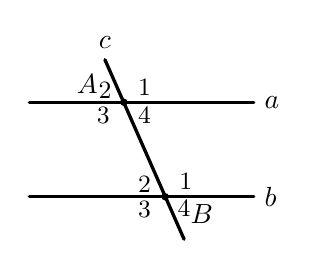
\begin{tikzpicture}[scale=0.75, line cap=round, line join=round]
  \draw[very thick] (-1.9, 0.9) -- (1.9, 0.9) node[right] {$a$};
  \draw[very thick] (-1.9, -0.7) -- (1.9, -0.7) node[right] {$b$};
  \coordinate (A) at (-0.3, 0.9);
  \coordinate (B) at (0.4, -0.7);
  \draw[very thick] ($ (A) + (-0.32, 0.72) $) node[above] {$c$} -- ($ (B) + (0.32, -0.72) $);
  \fill (A) circle (1.8pt);
  \fill (B) circle (1.8pt);
  \node at ($ (A) + (-0.62, 0.30) $) {$A$};
  \node at ($ (B) + (0.62, -0.30) $) {$B$};
  \node at ($ (A) + (0.35, 0.25) $) {\small $1$};
  \node at ($ (A) + (-0.32, 0.20) $) {\small $2$};
  \node at ($ (A) + (-0.35, -0.22) $) {\small $3$};
  \node at ($ (A) + (0.35, -0.22) $) {\small $4$};
  \node at ($ (B) + (0.35, 0.25) $) {\small $1$};
  \node at ($ (B) + (-0.35, 0.20) $) {\small $2$};
  \node at ($ (B) + (-0.35, -0.22) $) {\small $3$};
  \node at ($ (B) + (0.32, -0.20) $) {\small $4$};
\end{tikzpicture}
\end{minipage}

\newpage
\noindent\textbf{\large PHẦN II. Câu trắc nghiệm đúng sai (2,0 điểm).}
\vspace{0.5mm}

\noindent\textit{Thí sinh trả lời từ câu 13 đến câu 14. Trong mỗi ý a), b), c), d) ở mỗi câu, thí sinh chọn đúng hoặc sai.}

\vspace{1mm}
\noindent\textbf{Câu 13.} Cho các số thực $x = -\sqrt{7}$; $y = \dfrac{7}{11}$; $z = -2,6$; $t = \left|-\dfrac{5}{2}\right|$.\\
\begin{tabularx}{\linewidth}{X X}
\textbf{a)} $x$ là số vô tỉ. & \textbf{b)} $y = 0,6(3)$. \\
\textbf{c)} $z < x < t$. & \textbf{d)} Tổng các giá trị của $m$ thỏa mãn $|m + 1| = t$ bằng $-2$.
\end{tabularx}

\vspace{1mm}
\noindent
\begin{minipage}[m]{0.65\linewidth}
\textbf{Câu 14.} Cho hình bên, đường thẳng $c$ cắt hai đường thẳng $a, b$ lần lượt tại $M, N$; biết $\widehat{M}_2 = 115^\circ$ và $\widehat{N}_1 = 65^\circ$.\\
\textbf{a)} $\widehat{M}_1$ và $\widehat{M}_2$ là hai góc kề bù.\\
\textbf{b)} $\widehat{M}_1$ và $\widehat{N}_1$ là hai góc so le trong.\\
\textbf{c)} $a \parallel b$.\\
\textbf{d)} Tia phân giác của góc $M_3$ cắt đường thẳng $b$ tại $P$. Khi đó $\widehat{MPN} = 32,5^\circ$.
\end{minipage}
\hfill
\begin{minipage}[m]{0.33\linewidth}
\centering
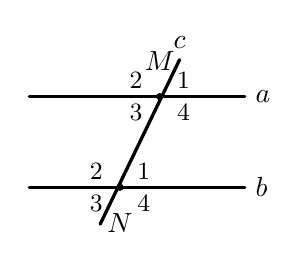
\begin{tikzpicture}[scale=0.72, line cap=round, line join=round]
  \draw[very thick] (-1.9, 0.9) -- (1.9, 0.9) node[right] {$a$};
  \draw[very thick] (-1.9, -0.7) -- (1.9, -0.7) node[right] {$b$};
  \coordinate (M) at (0.4, 0.9);
  \coordinate (N) at (-0.3, -0.7);
  \draw[very thick] ($ (N) - (0.35, 0.65) $) -- ($ (M) + (0.35, 0.65) $) node[above] {$c$};
  \fill (M) circle (1.8pt);
  \fill (N) circle (1.8pt);
  \node[above=6pt] at (M) {$M$};
  \node[below=6pt] at (N) {$N$};
  \node at ($ (M) + (0.42, 0.28) $) {\small $1$};
  \node at ($ (M) + (-0.42, 0.28) $) {\small $2$};
  \node at ($ (M) + (-0.42, -0.28) $) {\small $3$};
  \node at ($ (M) + (0.42, -0.28) $) {\small $4$};
  \node at ($ (N) + (0.42, 0.28) $) {\small $1$};
  \node at ($ (N) + (-0.42, 0.28) $) {\small $2$};
  \node at ($ (N) + (-0.42, -0.28) $) {\small $3$};
  \node at ($ (N) + (0.42, -0.28) $) {\small $4$};
\end{tikzpicture}
\end{minipage}

\vspace{1.5mm}
\noindent\textbf{\large PHẦN III. Câu trắc nghiệm trả lời ngắn (2,0 điểm).}
\vspace{0.5mm}

\noindent\textit{Thí sinh trả lời từ câu 15 đến câu 18.}

\vspace{1mm}
\noindent\textbf{Câu 15.} Tính giá trị của biểu thức $3\sqrt{16} - \sqrt{121}$.\hfill
\textbf{Câu 16.} Tìm $x$, biết $\dfrac{1}{2} - \dfrac{2}{3}x = -\dfrac{5}{6}$.

\vspace{1mm}
\noindent
\begin{minipage}[m]{0.65\linewidth}
\textbf{Câu 17.} Cho hình bên, biết $a \parallel b$, đường thẳng $c$ cắt $a, b$ lần lượt tại $H, K$ và $\widehat{H}_2 = 125^\circ$. Tính số đo góc $K_1$ (đơn vị: độ).\\
\textbf{Câu 18.} Một tấm bìa hình vuông có diện tích $75\text{ cm}^2$. Bạn Lan dán một sợi ruy băng sát theo bốn cạnh của tấm bìa. Tính độ dài sợi ruy băng (đơn vị: xăng-ti-mét, làm tròn đến hàng đơn vị).
\end{minipage}
\hfill
\begin{minipage}[m]{0.33\linewidth}
\centering
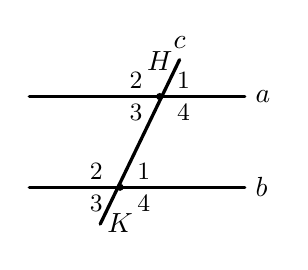
\begin{tikzpicture}[scale=0.72, line cap=round, line join=round]
  \draw[very thick] (-1.9, 0.9) -- (1.9, 0.9) node[right] {$a$};
  \draw[very thick] (-1.9, -0.7) -- (1.9, -0.7) node[right] {$b$};
  \coordinate (H) at (0.4, 0.9);
  \coordinate (K) at (-0.3, -0.7);
  \draw[very thick] ($ (K) - (0.35, 0.65) $) -- ($ (H) + (0.35, 0.65) $) node[above] {$c$};
  \fill (H) circle (1.8pt);
  \fill (K) circle (1.8pt);
  \node[above=6pt] at (H) {$H$};
  \node[below=6pt] at (K) {$K$};
  \node at ($ (H) + (0.42, 0.28) $) {\small $1$};
  \node at ($ (H) + (-0.42, 0.28) $) {\small $2$};
  \node at ($ (H) + (-0.42, -0.28) $) {\small $3$};
  \node at ($ (H) + (0.42, -0.28) $) {\small $4$};
  \node at ($ (K) + (0.42, 0.28) $) {\small $1$};
  \node at ($ (K) + (-0.42, 0.28) $) {\small $2$};
  \node at ($ (K) + (-0.42, -0.28) $) {\small $3$};
  \node at ($ (K) + (0.42, -0.28) $) {\small $4$};
\end{tikzpicture}
\end{minipage}

\vspace{1.5mm}
\noindent\textbf{\large PHẦN IV. Tự luận (3,0 điểm).}
\vspace{1mm}

\noindent\textbf{Câu 19 (1,0 điểm).} a) Tính hợp lí: $\dfrac{4}{9} \cdot \dfrac{13}{5} - \dfrac{4}{9} \cdot \dfrac{8}{5} + \dfrac{5}{9}$. \quad b) Tìm $x$, biết $\left(2x + \dfrac{1}{3}\right)^2 = \dfrac{25}{9}$.

\vspace{1mm}
\noindent\textbf{Câu 20 (1,0 điểm).} Thư viện trường có 240 quyển truyện. Lớp 7A mượn $\dfrac{1}{3}$ số truyện, lớp 7B mượn $\dfrac{3}{8}$ số truyện còn lại.\\
\textbf{a)} Sau khi hai lớp mượn, thư viện còn lại bao nhiêu quyển truyện?\\
\textbf{b)} Nhà trường mua thêm một số quyển truyện bằng $\dfrac{2}{5}$ số truyện còn lại ở câu a). Giá bìa mỗi quyển là $50\,000$ đồng và được giảm 12\% giá bìa. Tính số tiền nhà trường phải trả.

\vspace{1mm}
\noindent
\begin{minipage}[m]{0.64\linewidth}
\textbf{Câu 21 (1,0 điểm).} Cho hình bên, đường thẳng $AB$ cắt hai đường thẳng $mm'$ và $nn'$ lần lượt tại $A$ và $B$; biết $\widehat{mAB} = 110^\circ, \widehat{ABn} = 70^\circ$.\\
\textbf{a)} Chứng minh $mm' \parallel nn'$. \\
\textbf{b)} Đường thẳng $d$ đi qua $A$ và vuông góc với $mm'$, cắt $nn'$ tại $C$ (như hình bên). Chứng minh $d \perp nn'$ và tính số đo góc $BAC$.
\end{minipage}
\hfill
\begin{minipage}[m]{0.34\linewidth}
\centering
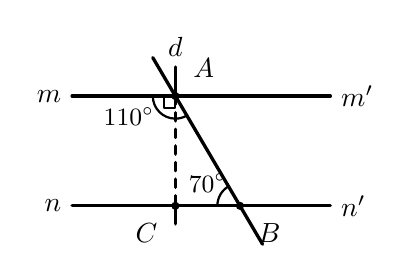
\begin{tikzpicture}[scale=0.82, line cap=round, line join=round]
  \coordinate (M) at (-2.0, 0.9);
  \coordinate (Mp) at (2.0, 0.9);
  \coordinate (N) at (-2.0, -0.8);
  \coordinate (Np) at (2.0, -0.8);
  \draw[very thick] (M) node[left] {$m$} -- (Mp) node[right] {$m'$};
  \draw[very thick] (N) node[left] {$n$} -- (Np) node[right] {$n'$};
  \coordinate (A) at (-0.4, 0.9);
  \coordinate (B) at (0.6, -0.8);
  \coordinate (C) at (-0.4, -0.8);
  \draw[very thick] ($ (A)!-0.35!(B) $) -- ($ (B)!-0.35!(A) $);
  \draw[very thick, dashed] (A) -- (C);
  \draw[very thick] ($ (A) + (0, 0.45) $) node[above] {$d$} -- (A);
  \draw[very thick] (C) -- ($ (C) + (0, -0.28) $);
  \draw[thick] (A) rectangle ++(-0.18, -0.18);
  \fill (A) circle (1.8pt) node[above right=3pt] {$A$};
  \fill (B) circle (1.8pt) node[below right=3pt] {$B$};
  \fill (C) circle (1.8pt) node[below left=3pt] {$C$};
  \draw[thick] ($ (A) + (-0.35, 0) $) arc (180:300:0.35);
  \node at ($ (A) + (-0.72, -0.32) $) {\small $110^\circ$};
  \draw[thick] ($ (B) + (-0.35, 0) $) arc (180:120:0.35);
  \node at (0.1, -0.45) {\small $70^\circ$};
\end{tikzpicture}
\end{minipage}

\vfill
\begin{center}
\textbf{--------- HẾT ---------}\\
\textit{(Giáo viên coi kiểm tra không giải thích gì thêm)}
\end{center}

\end{document}
